\documentclass[tikz,border=10pt]{standalone}
\usepackage{tikz}
\usetikzlibrary{shapes,arrows,positioning,calc,fit,backgrounds,shadows}

\begin{document}

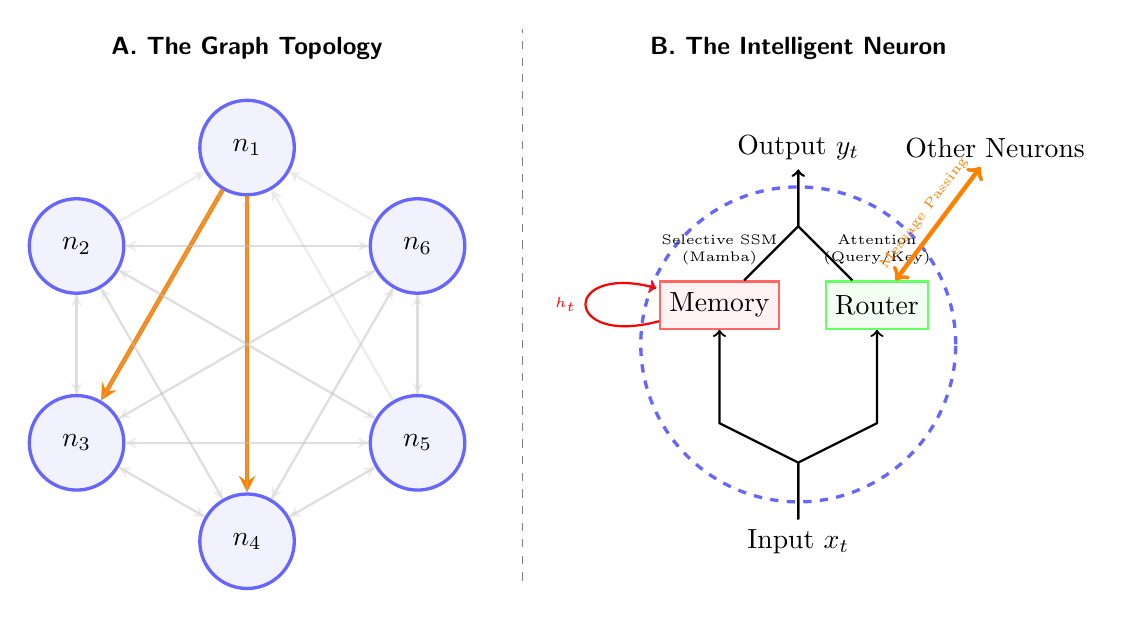
\begin{tikzpicture}[
    neuron/.style={circle, draw=blue!60, fill=blue!5, very thick, minimum size=1.2cm, inner sep=0pt},
    memory/.style={rectangle, draw=red!60, fill=red!5, thick, minimum size=0.6cm},
    comm/.style={rectangle, draw=green!60, fill=green!5, thick, minimum size=0.6cm},
    connection/.style={->, >=stealth, thick, gray!50},
    active_connection/.style={->, >=stealth, ultra thick, orange},
    label_text/.style={font=\sffamily\small\bfseries}
]

% --- MACRO VIEW: The Graph ---
\node[label_text, anchor=south] at (0, 3.5) {A. The Graph Topology};

% Create a circle of neurons
\def\n{6}
\def\radius{2.5}
\foreach \i in {1,...,\n} {
    \node[neuron] (N\i) at ({360/\n * (\i - 1) + 90}:\radius) {$n_\i$};
}

% Connect them (All-to-All simplified)
\foreach \i in {1,...,\n} {
    \foreach \j in {1,...,\n} {
        \ifnum\i=\j\else
            % Draw some active, some passive connections
            \ifnum\i=1
                \ifnum\j=3 \draw[active_connection] (N\i) -- (N\j); \fi
                \ifnum\j=4 \draw[active_connection] (N\i) -- (N\j); \fi
            \else
                \draw[connection, opacity=0.3] (N\i) -- (N\j);
            \fi
        \fi
    }
}

% --- MICRO VIEW: The Intelligent Neuron ---
\begin{scope}[shift={(7,0)}]
    \node[label_text, anchor=south] at (0, 3.5) {B. The Intelligent Neuron};
    
    % Neuron Boundary
    \node[neuron, minimum size=4cm, fill=white, dashed] (BigN) at (0,0) {};
    
    % Components
    \node[memory] (Mem) at (-1, 0.5) {Memory};
    \node[text width=1.5cm, align=center, font=\tiny] at (-1, 1.2) {Selective SSM\\(Mamba)};
    
    \node[comm] (Attn) at (1, 0.5) {Router};
    \node[text width=1.5cm, align=center, font=\tiny] at (1, 1.2) {Attention\\(Query/Key)};
    
    % Flow
    \node (Input) at (0, -2.5) {Input $x_t$};
    
    % Internal wiring
    \draw[->, thick] (Input) -- (0, -1.5) -- (-1, -1) -- (Mem);
    \draw[->, thick] (Input) -- (0, -1.5) -- (1, -1) -- (Attn);
    
    % Recurrence Loop (Memory)
    \draw[->, thick, red] (Mem) edge [loop left] node [left, font=\tiny] {$h_t$} (Mem);
    
    % Communication Lines
    \node (Others) at (2.5, 2.5) {Other Neurons};
    \draw[<->, ultra thick, orange] (Attn) -- (Others) node[midway, sloped, above, font=\tiny] {Message Passing};
    
    % Output
    \node (Output) at (0, 2.5) {Output $y_t$};
    \draw[->, thick] (Mem) -- (0, 1.5) -- (Output);
    \draw[->, thick] (Attn) -- (0, 1.5) -- (Output);
    
\end{scope}

% Separator
\draw[dashed, gray] (3.5, -3) -- (3.5, 4);

\end{tikzpicture}

\end{document}
